\chapter{Parallel Computing Fundamentals: Speedup, Laws, and Overhead}\label{ch:intro}
\begin{center}\small\textit{Why more workers do not always mean proportionally faster --- and what the math says about it.}\end{center}

\noindent\fbox{\parbox{\dimexpr\linewidth-2\fboxsep-2\fboxrule}{%
\textbf{From zero: no parallel background assumed.} We start with one cook in one kitchen (sequential execution). Adding cooks (cores) helps only if the recipe can be split, coordination is cheap, and no single step forces everyone to wait. This chapter makes that intuition precise.}}
\vspace{0.4em}

\section*{Learning Outcomes}
After this chapter you will be able to:
\begin{enumerate}[label=(L\arabic*)]
  \item define speedup, efficiency, and work/span;
  \item state and apply Amdahl's and Gustafson's laws;
  \item quantify overhead and its effect on scaling;
  \item use the Karp--Flatt metric and isoefficiency to diagnose poor scaling;
  \item distinguish strong versus weak scaling in experimental design.
\end{enumerate}

\section{Why Parallel? The Power Wall and the Free Lunch That Ended}
For decades single-core performance doubled every 18 months because transistors shrank and clocks rose. Around 2004 the \textbf{power wall} hit: $P\propto CV^{2}f$ and leakage meant higher $f$ melted the chip. Pollack's rule says performance $\propto\sqrt{\text{area}}$ --- doubling transistors in one core gives $\sim$40\% gain. Duplicating whole cores reuses the design and converts area into \textbf{thread-level parallelism (TLP)} with near-linear throughput if work is parallelisable.

Parallelism is not free. Splitting work creates \textbf{overhead}: communication, synchronisation, load imbalance, and extra computation. The central question is \emph{when does adding processors help, and by how much?} We need a yardstick.

\begin{definition}[Speedup and efficiency]\label{def:speedup}
Let $T_{1}$ be the time of the best sequential algorithm and $T_{p}$ the time on $p$ processors. Then
\[ S(p)=\frac{T_{1}}{T_{p}},\qquad E(p)=\frac{S(p)}{p}=\frac{T_{1}}{pT_{p}},\qquad \text{cost }C(p)=p\cdot T_{p}. \]
Linear speedup $S(p)=p\iff E(p)=1$. $S(p)>p$ (superlinear) usually means the sequential baseline was not the best, or cache effects.
\end{definition}

\begin{definition}[Work and span]\label{def:workspan}
\textit{Work} $T_{1}$ is total operations. \textit{Span} (critical-path length) $T_{\infty}$ is time on infinitely many processors. Any schedule satisfies $T_{p}\ge \max(T_{1}/p,\;T_{\infty})$ and parallelism $=T_{1}/T_{\infty}$ bounds the maximum useful $p$.
\end{definition}

\begin{example}[Work-span of parallel sum]
Summing $n$ numbers with a tree: $T_{1}=n$, $T_{\infty}=\log_{2}n$, parallelism $n/\log n$. With $p=n/\log n$, $T_{p}\approx\log n$; beyond that adding processors does not help.
\end{example}

\section{Amdahl's Law: The Fixed-Size Ceiling}
Assume fraction $f$ of work is perfectly parallelisable and $1-f$ is inherently serial.

\begin{theorem}[Amdahl's law]\label{thm:amdahl}
\[ S_{\text{Amdahl}}(p)=\frac{1}{(1-f)+f/p}\;\le\;\frac{1}{1-f}. \]
\end{theorem}
\begin{proof}
Normalise $T_{1}=1$. Serial part takes $1-f$; parallel part takes $f/p$. So $T_{p}=(1-f)+f/p$ and $S=1/T_{p}$. As $p\to\infty$, $S\to1/(1-f)$ regardless of $p$.
\end{proof}

If $f=0.9$, even $p=\infty$ gives $S\le10$. Doubling $p$ from $100$ to $1000$ moves $S$ from $9.17$ to $9.91$ --- diminishing returns are brutal. Amdahl tells us to attack the serial fraction first.

\begin{center}
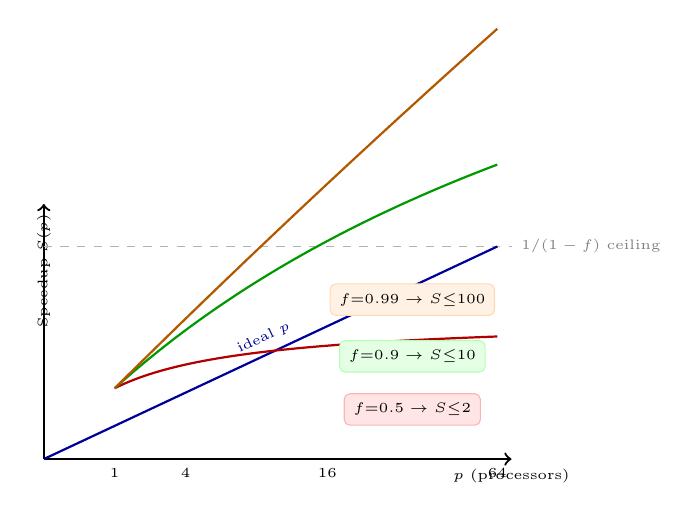
\begin{tikzpicture}[font=\scriptsize, scale=0.90]
\draw[->, thick] (0,0) -- (6.6,0) node[below, font=\tiny] {$p$ (processors)};
\draw[->, thick] (0,0) -- (0,3.6) node[left, rotate=90, font=\tiny] {Speedup $S(p)$};
\draw[dashed, gray!60] (0,3.0) -- (6.6,3.0) node[right, font=\tiny, text=gray] {$1/(1-f)$ ceiling};
\draw[thick, blue!60!black] (0,0) -- (6.4,3.0) node[midway, above, sloped, font=\tiny] {ideal $p$};
\foreach \f/\col/\off in {0.5/red!70!black/0.3, 0.9/green!60!black/0.5, 0.99/orange!70!black/0.0} {
  \draw[thick, \col] plot[domain=1:6.4, samples=80] (\x, {1/((1-\f)+\f/\x)});
}
\node[font=\tiny, fill=red!10, draw=red!30, rounded corners=2pt] at (5.2,0.7) {$f{=}0.5\to S{\le}2$};
\node[font=\tiny, fill=green!10, draw=green!30, rounded corners=2pt] at (5.2,1.45) {$f{=}0.9\to S{\le}10$};
\node[font=\tiny, fill=orange!10, draw=orange!30, rounded corners=2pt] at (5.2,2.25) {$f{=}0.99\to S{\le}100$};
\foreach \x/\lbl in {1/1, 2/4, 4/16, 6.4/64} \node[below, font=\tiny] at (\x,0) {\lbl};
\end{tikzpicture}
\end{center}
\captionof{figure}{Amdahl speedup versus $p$ for three parallel fractions; the horizontal asymptote is $1/(1-f)$.}
\label{fig:amdahl-curves}

\begin{remark}[Common pitfall]
$f$ must be measured for the \emph{best} sequential algorithm and the same problem size. Comparing against a slow baseline inflates $f$ and $S$.
\end{remark}

\section{Gustafson's Law: Scaled Speedup}
Amdahl fixes problem size (strong scaling). Gustafson observes users run \emph{larger} problems on bigger machines. Let $s=1-f$ and $f$ be fractions of \emph{parallel} execution time.

\begin{theorem}[Gustafson]\label{thm:gustafson}
\[ S_{\text{scaled}}(p)= (1-f)+f\cdot p = p - (p-1)(1-f). \]
If the problem scales so the serial fraction of parallel time stays constant, speedup grows linearly with $p$.
\end{theorem}
\noindent With $f=0.9$, $p=64$: $S_{\text{Amdahl}}\approx9.1$ but $S_{\text{scaled}}=57.7$. Both are correct under different assumptions. Report which you use.

\begin{center}
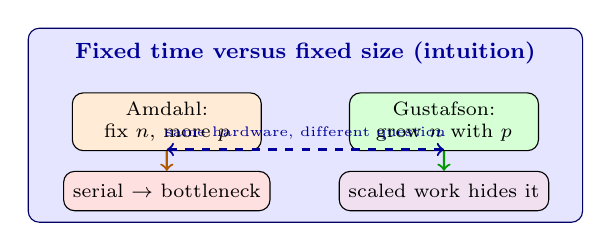
\begin{tikzpicture}[font=\scriptsize, scale=0.88]
\draw[fill=blue!10, draw=blue!40!black, rounded corners] (-0.2,-0.9) rectangle (7.8,1.9);
\node[font=\footnotesize\bfseries, text=blue!60!black] at (3.8,1.55) {Fixed time versus fixed size (intuition)};
\node[draw, fill=orange!16, minimum width=2.4cm, minimum height=0.7cm, align=center, rounded corners] (a) at (1.8,0.55) {Amdahl:\\fix $n$, more $p$};
\node[draw, fill=green!16, minimum width=2.4cm, minimum height=0.7cm, align=center, rounded corners] (g) at (5.8,0.55) {Gustafson:\\grow $n$ with $p$};
\node[draw, fill=red!12, minimum width=1.9cm, minimum height=0.5cm, align=center, rounded corners] (ser) at (1.8,-0.45) {serial $\to$ bottleneck};
\node[draw, fill=violet!12, minimum width=1.9cm, minimum height=0.5cm, align=center, rounded corners] (sca) at (5.8,-0.45) {scaled work hides it};
\draw[->, thick, orange!70!black] (a) -- (ser);
\draw[->, thick, green!60!black] (g) -- (sca);
\draw[<->, thick, blue!60!black, dashed] (1.8,0.15) -- (5.8,0.15) node[midway, above, font=\tiny] {same hardware, different question};
\end{tikzpicture}
\end{center}

Strong scaling ($n$ fixed) tests efficiency under control; weak scaling ($n\propto p$) tests ability to handle bigger science. A good paper reports both.

\section{Overhead, Efficiency, and Karp--Flatt}
Define total overhead $T_{O}(p)=pT_{p}-T_{1}$. Then $E=1/(1+T_{O}/T_{1})$. Useful taxonomy:

\begin{center}
\begin{tabular}{lp{7.8cm}}
\toprule Source & Example \\
\midrule Inter-process interaction & messages, cache coherence, lock contention \\
Idling & load imbalance, serial sections, synchronisation waits \\
Excess computation & redundant work for locality (e.g., halo recomputation) \\
\bottomrule
\end{tabular}
\end{center}

\begin{center}
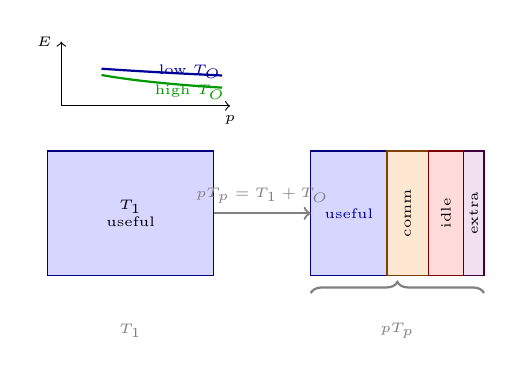
\begin{tikzpicture}[font=\scriptsize, scale=0.88]
% Stacked bar: T1 vs pTp
\draw[fill=blue!16, draw=blue!50!black] (0,0) rectangle (2.4,1.8) node[midway, font=\tiny, align=center] {$T_{1}$ \\ useful};
\draw[fill=blue!16, draw=blue!50!black] (3.8,0) rectangle (4.9,1.8) node[midway, font=\tiny, text=blue!60!black] {useful};
\draw[fill=orange!18, draw=orange!50!black] (4.9,0) rectangle (5.5,1.8) node[midway, font=\tiny, rotate=90] {comm};
\draw[fill=red!14, draw=red!50!black] (5.5,0) rectangle (6.0,1.8) node[midway, font=\tiny, rotate=90] {idle};
\draw[fill=violet!12, draw=violet!50!black] (6.0,0) rectangle (6.3,1.8) node[midway, font=\tiny, rotate=90] {extra};
\draw[->, thick, gray] (2.4,0.9) -- (3.8,0.9) node[midway, above, font=\tiny] {$pT_{p}=T_{1}+T_{O}$};
\draw[decorate, decoration={brace, amplitude=4pt}, thick, gray] (3.8,-0.25) -- (6.3,-0.25) node[midway, below, yshift=-0.25cm, font=\tiny] {$pT_{p}$};
\node[below, font=\tiny, text=gray] at (1.2,-0.55) {$T_{1}$};
% Efficiency vs p inset
\begin{scope}[shift={(0.2,2.45)}, scale=0.58]
\draw[->] (0,0) -- (4.2,0) node[below, font=\tiny] {$p$};
\draw[->] (0,0) -- (0,1.6) node[left, font=\tiny] {$E$};
\draw[thick, green!60!black] plot[domain=1:4, samples=40] (\x, {1/(1+0.3*\x)});
\draw[thick, blue!60!black] plot[domain=1:4, samples=40] (\x, {1/(1+0.08*\x)});
\node[font=\tiny, text=green!60!black] at (3.2,0.35) {high $T_{O}$};
\node[font=\tiny, text=blue!60!black] at (3.2,0.85) {low $T_{O}$};
\end{scope}
\end{tikzpicture}
\end{center}
\captionof{figure}{Left: work versus $pT_{p}$ including overhead. Right inset: efficiency decays as $p$ grows, faster with larger overhead.}
\label{fig:overhead-efficiency}

\begin{definition}[Karp--Flatt metric]\label{def:karpflatt}
Experimentally observed serial fraction:
\[ e(p)=\frac{1/S(p)-1/p}{1-1/p}. \]
If $e(p)$ grows with $p$, overhead is to blame; if $e(p)$ is flat $\approx1-f$, Amdahl's serial fraction dominates.
\end{definition}

\begin{definition}[Isoefficiency]\label{def:isoefficiency}
For a desired $E$, let $T_{O}(p,n)$ be overhead as function of $p$ and problem size $n$. Isoefficiency $n(p)$ solves $T_{O}/T_{1}= (1-E)/E =\text{const}$, i.e., how fast $n$ must grow to keep $E$ constant. Example: if $T_{O}=p\log p$ and $T_{1}=n$, then $n=\Theta(p\log p)$.
\end{definition}

\section{Putting It Together: Which Law to Use When?}
Use Amdahl to argue about \emph{latency} of a fixed job (user waiting). Use Gustafson to argue about \emph{throughput} of scaled science (bigger simulation). Use $T_{O}$, $e(p)$ and isoefficiency to decide whether to buy more cores or fix the algorithm. A parallel sort that is $0.9$ parallel on $n=10^{6}$ may be $0.99$ parallel on $n=10^{9}$ because the $O(n\log n)$ parallel work outgrows the $O(n)$ serial merge --- the fraction $f$ can be a function of $n$.

\begin{lstlisting}[language=Python, caption={Speedup, efficiency, and Karp--Flatt from measurements}, label={lst:speedup}]
def metrics(T1, Tp, p):
    S = T1 / Tp
    E = S / p
    e = (1/S - 1/p) / (1 - 1/p) if p > 1 else 0.0
    return S, E, e

# Strong scaling: n fixed, vary p
for p, Tp in [(1,120.0),(2,68.0),(4,40.0),(8,28.0)]:
    S,E,e = metrics(120.0, Tp, p)
    print(f"p={p} S={S:.2f} E={E:.2f} e={e:.3f}")
# e rising => overhead dominates; e flat => serial fraction dominates
\end{lstlisting}

\begin{lstlisting}[language=C, caption={Micro-benchmark skeleton for timing $T_{p}$ correctly}, label={lst:timing}]
double t0 = omp_get_wtime();
// warm cache, then barrier before timing
#pragma omp barrier
for (int r=0; r<REPS; r++) parallel_kernel(n);
#pragma omp barrier
double elapsed = (omp_get_wtime()-t0)/REPS;
// report min over REPS, pin threads, fix frequency, disable turbo
\end{lstlisting}

\begin{remark}[Measurement hygiene]
Pin threads, fix CPU frequency (disable turbo), warm up caches, take minimum over repetitions, and report variance. A speedup measured on a noisy laptop with thermal throttling is not science.
\end{remark}

\section{Numerical Synthesis}
Quick numbers cement the laws. For $f=0.9$, $T_{1}=100\,$s:
\begin{center}\small\begin{tabular}{c|c|c|c|c}
$p$ & $T_{p}$ Amdahl & $S$ & $E$ & $S_{\text{scaled}}$ (Gustafson)\\ \hline
1 & $100$ & $1.00$ & $1.00$ & $1.00$ \\
4 & $32.5$ & $3.08$ & $0.77$ & $3.70$ \\
16& $15.6$ & $6.40$ & $0.40$ & $14.5$ \\
64& $10.9$ & $9.14$ & $0.14$ & $57.7$ \\
\end{tabular}\end{center}
Amdahl predicts collapse of $E$ under strong scaling; Gustafson predicts healthy $E$ under weak scaling because $n$ grows. Real runs lie between, determined by $T_{O}(p,n)$.

\section{Exercises}
\begin{exercise}
A program has $f=0.85$ parallel fraction (Amdahl). Compute $S(4),S(16),S(64),S(\infty)$. If you double the parallel speedup from $10\times$ to $20\times$ only on the parallel part, what is the gain when $f=0.85$? Explain why investing in the serial part can beat doubling parallel speed.
\end{exercise}
\begin{exercise}
You measure $T_{1}=100\,\text{s}$, $T_{4}=30\,\text{s}$, $T_{8}=20\,\text{s}$. Compute $S,E$ and Karp--Flatt $e(4),e(8)$. Is the bottleneck serial fraction or overhead? Justify using the trend of $e(p)$.
\end{exercise}
\begin{exercise}
Derive Gustafson's law from the assumption that serial time is $1-f$ and parallel time is $f\cdot p$ after scaling $n$ with $p$. For $f=0.92$ and $p=32$, compute both Amdahl and Gustafson speedups and explain which is appropriate for (a) a fixed $4$K video encode, (b) a climate model where grid resolution scales with $p$.
\end{exercise}
\begin{exercise}
Suppose $T_{1}=c\,n\log n$ and $T_{O}=c_{1}p\log p + c_{2}p$ (reduction + barrier). Derive the isoefficiency function $n(p)$ to keep $E=0.8$. Is the algorithm highly scalable, modestly, or not scalable? What if $T_{O}=c_{1}p^{2}$?
\end{exercise}
\begin{exercise}
Strong versus weak scaling pitfall: a paper reports $E=0.92$ at $p=64$ under weak scaling and claims ``our system scales linearly.'' Design an experiment that could still reveal poor strong scaling, and explain why both numbers must be reported for a fair claim.
\end{exercise}

\section*{Chapter Notes}
Amdahl (1967) and Gustafson (1988) frame the oldest debate in parallel computing; Karp and Flatt (1990) gave the diagnostic $e(p)$. Overhead taxonomy and isoefficiency follow Grama, Gupta, Karypis and Kumar, \textit{Introduction to Parallel Computing} (2nd ed., Addison-Wesley). Work-span analysis is from Cormen et al., \textit{CLRS} (multithreaded model) and Blelloch. For measurement, see Hoefler and Belli, ``Scientific Benchmarking of Parallel Computing Systems'' (SC'15). Next we make parallelism concrete with threads.
